\scanpage{49}
% archive sheet number: 48

2.1.84

\deleted{On place sur $K$ des nouveaux sommets (d'ordre 2), de la façon suivante ; \deleted{Pour On \unsure{fixe|fera} par faces (soit $F$) de \unsure{laquelle|quelles}, on prend les sommets} arête par arête fermée.}

\deleted{a) On rajoute les pts de $K\cap L$ sur $\partial F$}

\deleted{b) Pour toute arête du nouveau complexe topologique $(\partial F,S\cap\partial F\cup(\partial F\cap L)$, \deleted{\unsure{on en}} distinguer}

\figure{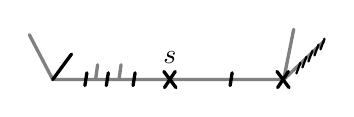
\begin{tikzpicture}[scale=.85,line cap=round]
\draw[gray,very thick] (-.35,.67)--(0,0)--(3.45,0)--(3.6,.75) (3.45,0)--(4.05,.57);
\draw[very thick] (0,0)--(.28,.38);
\foreach \x in {.48,.80,1.2,2.65}{\draw[very thick] (\x,-.09)--(\x+.03,.1);}
\foreach \x in {.64,.99}{\draw[gray,very thick] (\x,0)--(\x+.03,.22);}
\foreach \x in {1.75,3.44}{\draw[very thick] (\x-.08,-.12)--(\x+.08,.12) (\x-.09,.12)--(\x+.09,-.12);}
\node[above] at (1.75,.1){$s$};
\foreach \x in {0,.09,.18,.27,.36}{\draw[thick] (3.64+\x,.09+\x)--(3.7+\x,.25+\x);}
\end{tikzpicture}}

\figure{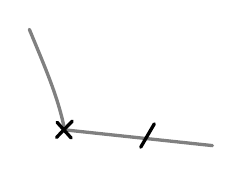
\begin{tikzpicture}[scale=.69,line cap=round]\draw[gray,very thick] (-.65,1.85) .. controls (-.34,1.1) and (-.12,.6) .. (0,0)--(2.72,-.29);\draw[very thick] (-.15,-.14)--(.14,.16) (-.14,.14)--(.12,-.15) (1.4,-.32)--(1.65,.11);\end{tikzpicture}}

\deleted{a) On rajoute les pts de $\bar a\cap L$ --- soit $\underline a'=(a,a\cap S(K)\cup a\cap L)$ le graphe-segment \inserted{top.} obtenu, soit $\alpha$ une arête de ce graphe.}

\deleted{(\uline{NB} \deleted{\unsure{Il}} Il y a au moins un \deleted{a) Si une des ext} élément de $a\cap L$ (\deleted{arête} ``sommet rouge'') sur $a$ distinct des extrémités, donc chaque arête $\alpha$ de $\underline a'$ \deleted{\unsure{cont}} a au moins une extrémité rouge, i.e. qui n'est pas une \deleted{sommet} \inserted{extrémité} de $\underline a$, et il y en a exactement deux qui n'en ont qu'une de rouge (l'autre étant verte)).}

\deleted{a) Sur ces dernières, on ne rajoute pas d'autre sommet \inserted{(sauf si l'extrémité en $a$ est un sommet de \unsure{$L$|la}} \deleted{\unsure{b)} Sur toute} Pour les autres arêtes, on \deleted{dis}rajoute des sommets (oranges) de la façon suivante}

\deleted{b) Si \deleted{les} les \inserted{deux} extrémités sont non critiques i.e. ne sont pas des sommets de $L$, on rajoute juste un sommet (le milieu)}

\deleted{c) \deleted{Si un} Pour les deux autres arêtes (cas d'une arête $\underline a$ ordinaire), de part et d'autre du pt critique \deleted{\unsure{$t$}} $s$, si $\nu(s)$ est son ordre, on dispose $\frac{\nu(s)}2$ pts rouges (si}
